\documentclass[11pt,a4paper]{article}

% ── Packages ──────────────────────────────────────────────
\usepackage[utf8]{inputenc}
\usepackage[T1]{fontenc}
\usepackage{amsmath,amssymb}
\usepackage{graphicx}
\usepackage{booktabs}
\usepackage[round]{natbib}
\usepackage{hyperref}
\usepackage[margin=2.5cm]{geometry}

% ── Title ─────────────────────────────────────────────────
\title{Affective Valence and Temporal Framing:\\
       A Computational Theory of Counterfactual Precision Redistribution}
\author{Mahault Albarracin}
\date{}

\begin{document}
\maketitle

\begin{abstract}
Emotions are temporally structured: regret concerns what has happened, anxiety concerns what will happen, and surprise concerns what is happening now. Within predictive processing, variational free energy (VFE) evaluates how well the agent's model fits past observations, while expected free energy (EFE) evaluates how well future observations will match preferences. We propose that this computational distinction provides a unified temporal taxonomy of affect: emotions inherit their temporal direction from whichever free energy quantity generates them. Building on this mapping, we formalise counterfactual temporal framing as the mechanism by which agents actively navigate the temporal structure of affect. Temporal framing is cast as policy selection within a partially observable Markov decision process, where each policy redistributes precision across temporal horizons via distinct transition matrices. We show that this redistribution emerges naturally from EFE minimisation: high prediction error favours future-oriented framing (prospective counterfactual simulation), while stable beliefs with high positive-belief precision favour past-oriented framing (autobiographical narrative stabilisation). A three-channel valence decomposition, separating backward (model valence), present (reward valence), and forward (action valence) components, provides a direct readout of temporal orientation at each timestep. Simulations demonstrate that healthy agents balance temporal orientations adaptively, with past-oriented framing serving as a preparatory step for present engagement. Chronic stress produces a pathological pattern: elevated future and past frame beliefs with depleted present engagement, persistent backward negative valence from chronic model-fit deterioration, and a self-amplifying cycle where precise future predictions are systematically violated by a volatile environment. We connect this framework to the mood--emotion timescale hierarchy, depression as failed temporal flexibility, and the broader project of temporal aiming in active inference.
\end{abstract}


\section{Introduction}\label{sec:introduction}

How do organisms decide where in time to direct their attention? A key insight of predictive processing is that affect is not a post-hoc label attached to perception but an integral part of the inference process itself \citep{barrett2017theory, seth2016interoceptive}. Valence, on this account, reflects the rate of change of the agent's model fit to its environment \citep{joffily2013emotional}: improving fit produces positive valence, deteriorating fit produces negative valence. This formulation grounds affect in the same variational free energy (VFE) quantity that drives perception and learning.

A complementary strand of work has shown that affect is also forward-looking. Expected free energy (EFE), the quantity minimised in active inference policy selection \citep{parr2022active}, evaluates how well future observations will match preferences under each available policy. \citet{hesp2021deeply} showed that the ``affective charge'' of policy revision, that is, the degree to which the agent shifts probability toward better policies, constitutes a forward-looking valence signal. \citet{pattisapu2024free} extended the affective readout to include a present-oriented reward prediction error channel, completing a three-channel architecture spanning backward, present, and forward temporal orientations.

These contributions establish that affect has temporal structure. Yet no existing paper formally unifies the VFE/EFE distinction into a temporal taxonomy of emotion, nor provides a computational model of how organisms \emph{actively navigate} this temporal structure. \citet{hinrichs2025temporal} introduced ``temporal aiming'' in the context of dyadic interaction, showing how agents coordinate their temporal orientations during social exchange. However, the single-agent computational mechanism, the process by which an individual agent selects which temporal horizon of free energy dominates its affective signal, remains unaddressed.

This paper fills both gaps. We formally propose the VFE/EFE temporal mapping as a unified theory of affective temporal direction (\S\ref{sec:temporal_structure}), derive a three-channel valence architecture that decomposes affect into its temporal components (\S\ref{sec:three_channel}), and formalise counterfactual temporal framing as precision redistribution across temporal horizons (\S\ref{sec:counterfactual}). Temporal framing is not a separate cognitive function bolted onto inference; it \emph{emerges} from EFE minimisation given the right generative model structure. We demonstrate this with simulations of past-oriented framing (\S\ref{sec:past}), future-oriented framing (\S\ref{sec:future}), and the pathological case of chronic stress as maladaptive temporal fixation (\S\ref{sec:chronic_stress}).

The generative model is shared with a companion paper on bipolar disorder \citep{albarracin2026bipolar}, which focuses on clinical phenotypes arising from parameter variation along energy, interoception, and granularity dimensions. The present paper abstracts away from those clinical particulars to address the general computational mechanism of temporal affect regulation.


\section{The Temporal Structure of Free Energy}\label{sec:temporal_structure}

\subsection{VFE as Backward-Looking Evaluation}\label{sec:vfe}

Variational free energy provides the fundamental backward-looking evaluation in active inference. For a generative model $p(o, s)$ with approximate posterior $q(s)$ over hidden states $s$ given observations $o$:
\begin{equation}
    F = \underbrace{-\mathbb{E}_{q(s)}[\ln p(o \mid s)]}_{\text{accuracy}} + \underbrace{D_{\mathrm{KL}}[q(s) \,\|\, p(s)]}_{\text{complexity}}
\end{equation}
$F$ evaluates how well the \emph{current} model fits \emph{past} observations: accuracy measures the expected log-likelihood of what has already been observed, while complexity penalises deviation from prior beliefs. Minimising $F$ with respect to $q(s)$ is perception; minimising $F$ with respect to $p(o,s)$ is learning.

\citet{joffily2013emotional} showed that the temporal derivative of $F$ provides a natural valence signal:
\begin{equation}
    -\frac{dF}{dt}: \quad \text{rate of model improvement}
\end{equation}
Decreasing $F$ (improving model fit) produces positive valence; increasing $F$ produces negative valence. This is inherently backward-looking: it evaluates the \emph{trajectory} of model fit over recent observations.

The second temporal derivative $-d^2F/dt^2$ further differentiates affective states by their dynamics. When both $dF$ and $d^2F$ are negative, the model fit is improving at an accelerating rate, corresponding to \textbf{hope}. When $dF$ is negative but $d^2F$ is positive, improvement is decelerating and stabilising into a good state, corresponding to \textbf{happiness}. Conversely, when both are positive, model fit is worsening at an accelerating rate, corresponding to \textbf{fear}, while negative $d^2F$ with positive $dF$ indicates stabilisation into a bad state, corresponding to \textbf{unhappiness}. Sign changes in $dF$ mark affective transitions: a shift from positive to negative $dF$ corresponds to \textbf{relief}, while a shift from negative to positive corresponds to \textbf{disappointment}. This taxonomy derives entirely from the dynamics of a single backward-looking quantity.

\subsection{EFE as Forward-Looking Evaluation}\label{sec:efe}

Expected free energy provides the complementary forward-looking evaluation. For a policy $\pi$ that produces predicted future observations:
\begin{equation}
    G(\pi) = \sum_m \left[\underbrace{D_{\mathrm{KL}}[q(o_m \mid \pi) \,\|\, p(o_m \mid C_m)]}_{\text{risk}_m} + \underbrace{\mathbb{E}_{q(s)}[H[p(o_m \mid s)]]}_{\text{ambiguity}_m}\right]
\end{equation}
where the sum ranges over observation modalities $m$, $q(o_m \mid \pi)$ is the predicted observation distribution under policy $\pi$, and $p(o_m \mid C_m)$ encodes preferences. Risk measures the divergence between predicted and preferred observations; ambiguity measures the expected entropy of the observation model.

$G(\pi)$ evaluates how well \emph{future} observations will match preferences: it asks not ``did I predict well?'' (VFE) but ``will I predict well?'' (EFE). This temporal complement is the foundation of the mapping we propose.

\subsection{The VFE/EFE Temporal Mapping}\label{sec:temporal_mapping}

We propose that emotions inherit their temporal direction from whichever free energy quantity generates them. This yields a systematic taxonomy.

\paragraph{Backward (VFE-generated).} Emotions grounded in the evaluation of past model fit include \emph{regret} (VFE higher than counterfactual alternative), \emph{guilt} (VFE elevated due to own action), \emph{shame} (VFE elevated due to social model violation), \emph{pride} (VFE lower than expected), and \emph{gratitude} (VFE reduction attributed to another agent).

\paragraph{Present ($-dF/dt$ or RPE).} Emotions grounded in the rate of change at the current moment include \emph{joy} (rapid VFE decrease), \emph{anger} (VFE increase attributed to external agent), \emph{disgust} (VFE increase in interoceptive modality), and \emph{surprise} (large absolute $\Delta F$).

\paragraph{Forward (EFE-generated).} Emotions grounded in the evaluation of expected future performance include \emph{hope} (low EFE under preferred policy), \emph{fear} (high EFE across all policies), \emph{anxiety} (high EFE with high ambiguity), and \emph{anticipation} (low EFE with low ambiguity).

\paragraph{Transitional (VFE vs prior EFE).} Emotions that arise from comparing current VFE with previously computed EFE include \emph{relief} (VFE lower than EFE had predicted), \emph{disappointment} (VFE higher than EFE had predicted), and \emph{satisfaction} (VFE confirms low EFE prediction).

This mapping extends the appraisal-theoretic classification of \citet{smith1985patterns} and the OCC model of \citet{ortony1988cognitive} by grounding the temporal dimension in the formal distinction between variational and expected free energy, rather than in folk-psychological temporal labels.

\subsection{Counterfactual Emotions and Temporal Simulation}\label{sec:counterfactual_emotions}

A particularly revealing class of emotions requires maintaining beliefs about unchosen policies. \citet{hesp2020sophisticated} showed that \emph{sophisticated} affective inference involves evaluating counterfactual trajectories: the agent computes what \emph{would have} happened under alternative policies, and the divergence between actual and counterfactual VFE generates emotions like regret and relief.

Formally, regret at time $t$ is:
\begin{equation}
    \text{Regret} = F_{\text{actual}}(t) - \min_{\pi'} F_{\text{counterfactual}}(t \mid \pi')
\end{equation}
Computing $F_{\text{counterfactual}}$ requires running the generative model \emph{offline}, simulating what would have happened under the unchosen policy. This is exactly what temporal framing does: the agent simulates past states (RECALL) or future states (FUTURATE) by running its generative model in a mode decoupled from current sensory input. Counterfactual emotions thus require the same computational machinery as temporal framing, suggesting that temporal framing may be the general mechanism and counterfactual emotions its specific affective products.


\section{Three-Channel Valence as Temporal Derivative Decomposition}\label{sec:three_channel}

\subsection{Three Readings from the Inference Pipeline}\label{sec:pipeline}

Each valence channel reads from a different point in the agent's processing loop:
\begin{equation}
    \text{observation} \to \underbrace{\text{belief update}}_{\to\, v_{\text{model}}} \to \underbrace{\text{EFE recomputation}}_{\to\, v_{\text{reward}}} \to \underbrace{\text{policy update}}_{\to\, v_{\text{action}}}
\end{equation}
This sequential structure means the three channels are not independent measurements of the same quantity but successive evaluations at increasing temporal remove from the current observation.

\subsection{Channel 1: Model Valence $v_{\text{model}}$ (Backward)}\label{sec:v_model}

Following \citet{joffily2013emotional}, model valence tracks the rate of change of variational free energy:
\begin{equation}
    v_{\text{model}} = \tanh\!\left(\frac{-\Delta F}{\tau_{\text{model}}}\right)
\end{equation}
where $\Delta F = F(t) - F(t{-}1)$. Decreasing free energy (improving model fit) produces positive valence; increasing free energy produces negative valence.

This channel has a natural functional role: it drives the learning rate. Persistently negative $v_{\text{model}}$ signals that the model is deteriorating, which should accelerate learning ($\sigma_{\text{eff}} = \sigma \times \exp(-\alpha \cdot v_{\text{model}})$). Its temporal character is strictly backward: it evaluates the current state relative to the model's past predictions.

\subsection{Channel 2: Reward Valence $v_{\text{reward}}$ (Present)}\label{sec:v_reward}

Following \citet{pattisapu2024free}, reward valence captures the momentary reward prediction error:
\begin{equation}
    v_{\text{reward}} = \tanh\!\left(\frac{U - \mathbb{E}[U]}{\tau_{\text{reward}}}\right)
\end{equation}
where $U = \sum_m \log P(o_m \mid C_m)$ is the utility of the observed outcome and $\mathbb{E}[U] = \sum_m \sum_o Q(o_m) \log P(o_m \mid C_m)$ is the expected utility under predicted observations.

This channel drives preference monitoring: chronic negative $v_{\text{reward}}$ signals that the agent's preferences ($\mathbf{C}$ vectors) may be unrealistic. Its temporal character is present-oriented: it evaluates \emph{this} observation relative to what was expected.

\subsection{Channel 3: Action Valence $v_{\text{action}}$ (Forward)}\label{sec:v_action}

Following \citet{hesp2021deeply}, action valence captures the affective charge of policy revision:
\begin{equation}
    v_{\text{action}} = \tanh\!\left(\frac{\text{AC}}{\tau_{\text{action}}}\right), \qquad \text{AC} = (\boldsymbol{\pi}_{t-1} - \boldsymbol{\pi}_t) \cdot \mathbf{G}
\end{equation}
where $\boldsymbol{\pi}$ is the policy distribution and $\mathbf{G}$ the expected free energy vector. Positive affective charge indicates the agent is shifting probability \emph{away from} high-EFE policies (planning improvement); negative charge indicates deterioration.

This channel drives precision updating: positive $v_{\text{action}}$ increases the effective inverse temperature $\bar{\beta}$ (more decisive policy selection), while negative $v_{\text{action}}$ decreases it (more exploratory). Its temporal character is forward-looking: it evaluates whether the agent's \emph{planning} is improving.

\subsection{Composite Valence and Channel Disagreement}\label{sec:composite}

The three channels combine into a single bounded signal:
\begin{equation}
    V = \tanh(v_{\text{model}} + v_{\text{reward}} + v_{\text{action}})
\end{equation}

When channels agree, the affective signal is unambiguous: genuine satisfaction when all are positive, or genuine distress when all are negative. When they disagree, the resulting states are informationally rich. A state of \emph{productive failure} arises when $v_{\text{model}} < 0$ and $v_{\text{action}} > 0$: the current observation was bad, but the agent found a better plan, corresponding to learning from mistakes. \emph{Unsettling success} occurs when $v_{\text{reward}} > 0$ but $v_{\text{action}} < 0$: the outcome was good, but the planning landscape worsened, suggesting that good fortune may be unsustainable. \emph{Dawning anxiety} appears when $v_{\text{model}} \approx 0$, $v_{\text{reward}} \approx 0$, and $v_{\text{action}} < 0$: nothing has happened, but plans are deteriorating, producing the computational signature of anticipatory dread.

\subsection{Temporal Orientation as Normalised Channel Contribution}\label{sec:temporal_orientation}

We define the temporal orientation at each timestep as the normalised absolute channel contribution:
\begin{equation}
    \phi_{\text{dir}}(t) = \frac{|v_{\text{dir}}(t)|}{|v_{\text{model}}(t)| + |v_{\text{reward}}(t)| + |v_{\text{action}}(t)| + \epsilon}
\end{equation}
and the \emph{backward--forward conflict rate} as the fraction of timesteps where $v_{\text{model}}$ and $v_{\text{action}}$ have opposite signs.

Different emotions have characteristic temporal orientation profiles. Rumination is backward-dominated with high conflict; impulsivity is present-dominated with low conflict; anxiety is forward-dominated with high conflict. This connects the three-channel architecture back to the VFE/EFE temporal mapping of \S\ref{sec:temporal_mapping}: the channels provide a continuous, per-timestep readout of which temporal horizon currently dominates the agent's affect.


\section{Counterfactual Temporal Framing as Precision Redistribution}\label{sec:counterfactual}

\subsection{Attention as Precision}\label{sec:attention_precision}

In predictive processing, attention is precision weighting on prediction errors \citep{feldman2010attention}. Precision determines \emph{which} errors are amplified and therefore \emph{which} beliefs update. We extend this principle to the temporal domain: \emph{temporal precision} determines which temporal \emph{horizon} of predictions matters. Attending to the past (reminiscence) amplifies prediction errors from memory retrieval; attending to the future (prospection) amplifies prediction errors from simulated outcomes.

\subsection{The Generative Model: Temporal Frame as Hidden State}\label{sec:gen_model}

We adopt the factored POMDP structure described in detail in our companion paper \citep{albarracin2026bipolar}. The hidden state $s = (v, e, f)$ is factored into three dimensions: \textbf{valence} $v \in \{0, \ldots, K{-}1\}$ (affective state at granularity $K$), \textbf{energy} $e \in \{0, \ldots, M{-}1\}$ (interoceptive resource estimate), and \textbf{temporal frame} $f \in \{\textsc{past}, \textsc{present}, \textsc{future}\}$ (currently active counterfactual orientation).

Critically, $f$ is a genuinely hidden state that the agent \emph{infers}, not a label it assigns. Temporal orientation is something the agent believes about \emph{itself}, updated through the same Bayesian machinery as all other hidden states. The posterior frame belief $q(f \mid o)$, obtained by marginalising $q(v, e, f \mid o)$ over valence and energy, provides a direct readout of the agent's believed temporal orientation.

\subsection{$\mathbf{B}_{\text{frame}}$ Matrices as Temporal Precision Operators}\label{sec:b_frame}

Each action defines a distinct transition structure $\mathbf{B}_a = \mathbf{B}_v^{(a)} \otimes \mathbf{B}_e^{(a)} \otimes \mathbf{B}_f^{(a)}$. The frame transition matrices $\mathbf{B}_f^{(a)}$ function as \emph{temporal precision operators}, redistributing probability across temporal frames and thereby determining which horizon the agent attends to.

\paragraph{RECALL.} The frame matrix $\mathbf{B}_f^{\textsc{recall}}$ assigns 70\% self-transition to \textsc{past}, allocating precision to past-generated internal states; autobiographical memory retrieval becomes ``attending to the past.'' Simultaneously, $\mathbf{B}_v^{\textsc{recall}}$ pulls the valence state toward the prior $\mathbf{D}$ with strength $\alpha = \sigma(\pi_{\text{pos}} - \theta)$, re-accessing the agent's self-model.

\paragraph{ENGAGE.} The frame matrix $\mathbf{B}_f^{\textsc{engage}}$ assigns 75\% self-transition to \textsc{present}, maintaining precision on current sensory input through standard perception--action coupling.

\paragraph{FUTURATE.} The frame matrix $\mathbf{B}_f^{\textsc{futurate}}$ assigns 90\% self-transition to \textsc{future}, allocating precision to anticipated future states. The high absorptivity reflects ``narrative inertia'': once engaged in prospective simulation, the agent tends to persist. Simultaneously, $\mathbf{B}_v^{\textsc{futurate}}$ pulls valence toward the solution state $K{-}1$, imagining the best outcome.

\paragraph{REST.} The frame matrix $\mathbf{B}_f^{\textsc{rest}}$ assigns 50--60\% to \textsc{present}, releasing frame commitment and allowing the temporal orientation to reset.

\subsection{Counterfactual Simulation as Decoupled Inference}\label{sec:decoupled}

Standard inference updates beliefs about the current state given current observations. Temporal framing extends this by performing inference about \emph{counterfactual} states, that is, states not currently generating observations.

When the agent selects RECALL, $\mathbf{B}_v^{\textsc{recall}}$ pulls beliefs toward the prior $\mathbf{D}$: the agent is re-accessing its past self-model, running inference on what its affective state \emph{was} (or what it \emph{could have been} had things gone differently). When the agent selects FUTURATE, $\mathbf{B}_v^{\textsc{futurate}}$ pulls beliefs toward the solution state: the agent is imagining its best possible future, running inference on what its affective state \emph{will be} under the most optimistic scenario.

This constitutes ``mentalisation'' in the active inference sense: inference running offline, decoupled from current sensory evidence. Both autobiographical memory retrieval and prospective simulation engage overlapping neural substrates associated with the default mode network, consistent with deep temporal models of offline inference \citep{friston2018deep} and suggesting that these are two instances of the same counterfactual inference mechanism.

\subsection{EFE as Natural Temporal Routing}\label{sec:efe_routing}

The core theoretical claim of this paper is that temporal framing is not a separate cognitive function but \emph{emerges} from EFE minimisation given the generative model structure described above.

Each action has different risk and ambiguity because of its different $\mathbf{B}$ matrices. The agent's context, including its current VFE, beliefs, and energy level, determines which temporal orientation is EFE-favoured:
\begin{equation}
    G(a) = \sum_m \left[\text{risk}_m(a) + \text{ambiguity}_m(a)\right]
\end{equation}

When VFE is high and beliefs are far from preferred, FUTURATE wins because $\mathbf{B}_v^{\textsc{futurate}}$ pulls most strongly toward the preferred (solution) state, yielding the largest risk reduction in the valence modality. When the agent's model fits well and positive self-beliefs enable effective recall, RECALL wins by maintaining affect via the prior pull with minimal energy cost. When energy is depleted, REST wins because $\mathbf{B}_e^{\textsc{rest}}$ restores energy, yielding the lowest energy-modality risk. The standard softmax policy selection $\pi(a) \propto \exp(-\gamma \cdot G(a))$ then naturally routes the agent toward the appropriate temporal frame. No temporal routing heuristic is needed; the structure is already in the generative model.

\subsection{Temporal Framing and the Emotion--Action--Inference Loop}\label{sec:loop}

The complete cycle linking temporal framing to affect is:
\begin{equation}
    \text{EFE} \to \text{policy} \to \text{action} \to \text{observation} \to \text{VFE} \to \text{valence} \to \text{precision} \to \text{EFE}
\end{equation}

Temporal framing policies modify \emph{which part of this loop dominates}: RECALL amplifies the VFE $\to v_{\text{model}}$ path (backward evaluation), ENGAGE amplifies the observation $\to v_{\text{reward}}$ path (present evaluation), and FUTURATE amplifies the EFE $\to v_{\text{action}}$ path (forward evaluation).

This creates two dynamical regimes. In \emph{self-regulation}, the loop is homeostatic: negative valence increases learning rate, which improves the model, which produces positive valence \citep{joffily2013emotional}. In \emph{self-amplification}, the loop becomes pathological: temporal framing locks into a single mode, precision on that mode's prediction errors increases, and the agent cannot escape the attractor. The transition from self-regulation to self-amplification is the computational mechanism of chronic stress (\S\ref{sec:chronic_stress}).


\section{Past-Oriented Framing: Narrative Stabilisation}\label{sec:past}

\subsection{Mechanism of RECALL}\label{sec:recall_mechanism}

The RECALL policy redistributes precision toward past-generated internal states via two coupled mechanisms. First, $\mathbf{B}_f^{\textsc{recall}}$ shifts frame beliefs toward \textsc{past} (70\% self-transition). Second, $\mathbf{B}_v^{\textsc{recall}}$ pulls the valence state toward the prior $\mathbf{D}$ with strength $\alpha = \sigma(\pi_{\text{pos}} - \theta)$.

The sigmoid gating function produces an all-or-nothing effect at the threshold $\pi_{\text{pos}} \approx 2.0$. When $\pi_{\text{pos}}$ is high ($\alpha \to 1$), RECALL effectively generates positive counterfactuals grounded in a confident self-model. When $\pi_{\text{pos}}$ is low ($\alpha \approx 0.12$), RECALL is biologically ineffective: the agent cannot access specific positive autobiographical memories, consistent with the ``overgeneral autobiographical memory'' observed in depression \citep{williams2007autobiographical}.

The energy cost of RECALL is minimal. Running the generative model offline on past states is computationally cheap relative to active environmental engagement. This gives RECALL a natural advantage in the EFE decomposition: low valence risk (via the prior pull) combined with low energy risk.

\subsection{RECALL Supports Engagement}\label{sec:recall_engagement}

A critical claim of this paper is that past-oriented framing is \emph{preparatory}: narrative consolidation enables action rather than substituting for it. The RECALL$\to$ENGAGE pipeline operates as follows: RECALL stabilises beliefs by pulling toward the prior, which lowers VFE. Lower VFE means the ENGAGE policy becomes more competitive (its risk terms decrease when beliefs are closer to preferred states). The agent naturally transitions from RECALL to ENGAGE as its beliefs stabilise.

Simulation evidence supports this claim (Figure~\ref{fig:framing_dynamics}d, e). Action transition matrices show a substantial RECALL$\to$ENGAGE path in healthy agents. Post-action valence stability analysis reveals that RECALL produces lower 5-step valence variance than REST or FUTURATE, confirming that RECALL \emph{stabilises} affect rather than merely boosting it. This stabilisation is the computational basis for the claim: by anchoring beliefs in positive prior expectations (via the $\mathbf{B}_v^{\textsc{recall}}$ pull toward $\mathbf{D}$), RECALL reduces the volatility of subsequent prediction errors, creating a more stable platform for engagement.

\subsection{When Past Framing Fails: Feedback Reliance}\label{sec:feedback_reliance}

When $\pi_{\text{pos}}$ is low, $\alpha \approx 0.12$ and RECALL becomes biologically ineffective. The EFE landscape shifts: RECALL's predicted valence gain is diminished while its (minimal) energy cost remains unchanged. REST, which reliably restores energy and drifts valence toward neutral, becomes the dominant policy by default.

Figure~\ref{fig:feedback_reliance} demonstrates this pattern by comparing two profiles with identical reward sensitivity ($c_{\text{scale}} = 1.0$), granularity ($K = 8$), and interoceptive precision ($\omega_e = 5.0$), differing only in positive-belief precision: healthy ($\pi_{\text{pos}} = 5.0$) versus recall-impaired ($\pi_{\text{pos}} = 0.2$). The recall-impaired agent shows a dramatic collapse of RECALL utilisation (from 41\% to 7\%), with compensatory REST increase (59\% to 87\%) and emergent FUTURATE selection (6\% vs 0\%).

The emergent FUTURATE selection demonstrates a partial compensatory mechanism: when backward-looking counterfactuals fail, the agent can redirect toward forward-looking strategies if reward sensitivity is intact. In the full depressive profile (where $c_{\text{scale}} = 0.1$), this compensatory pathway is also blocked by anhedonia, producing a double dissociation: recall impairment removes the backward regulatory mechanism, while anhedonia removes the forward compensatory pathway.

\begin{figure}[htbp]
    \centering
    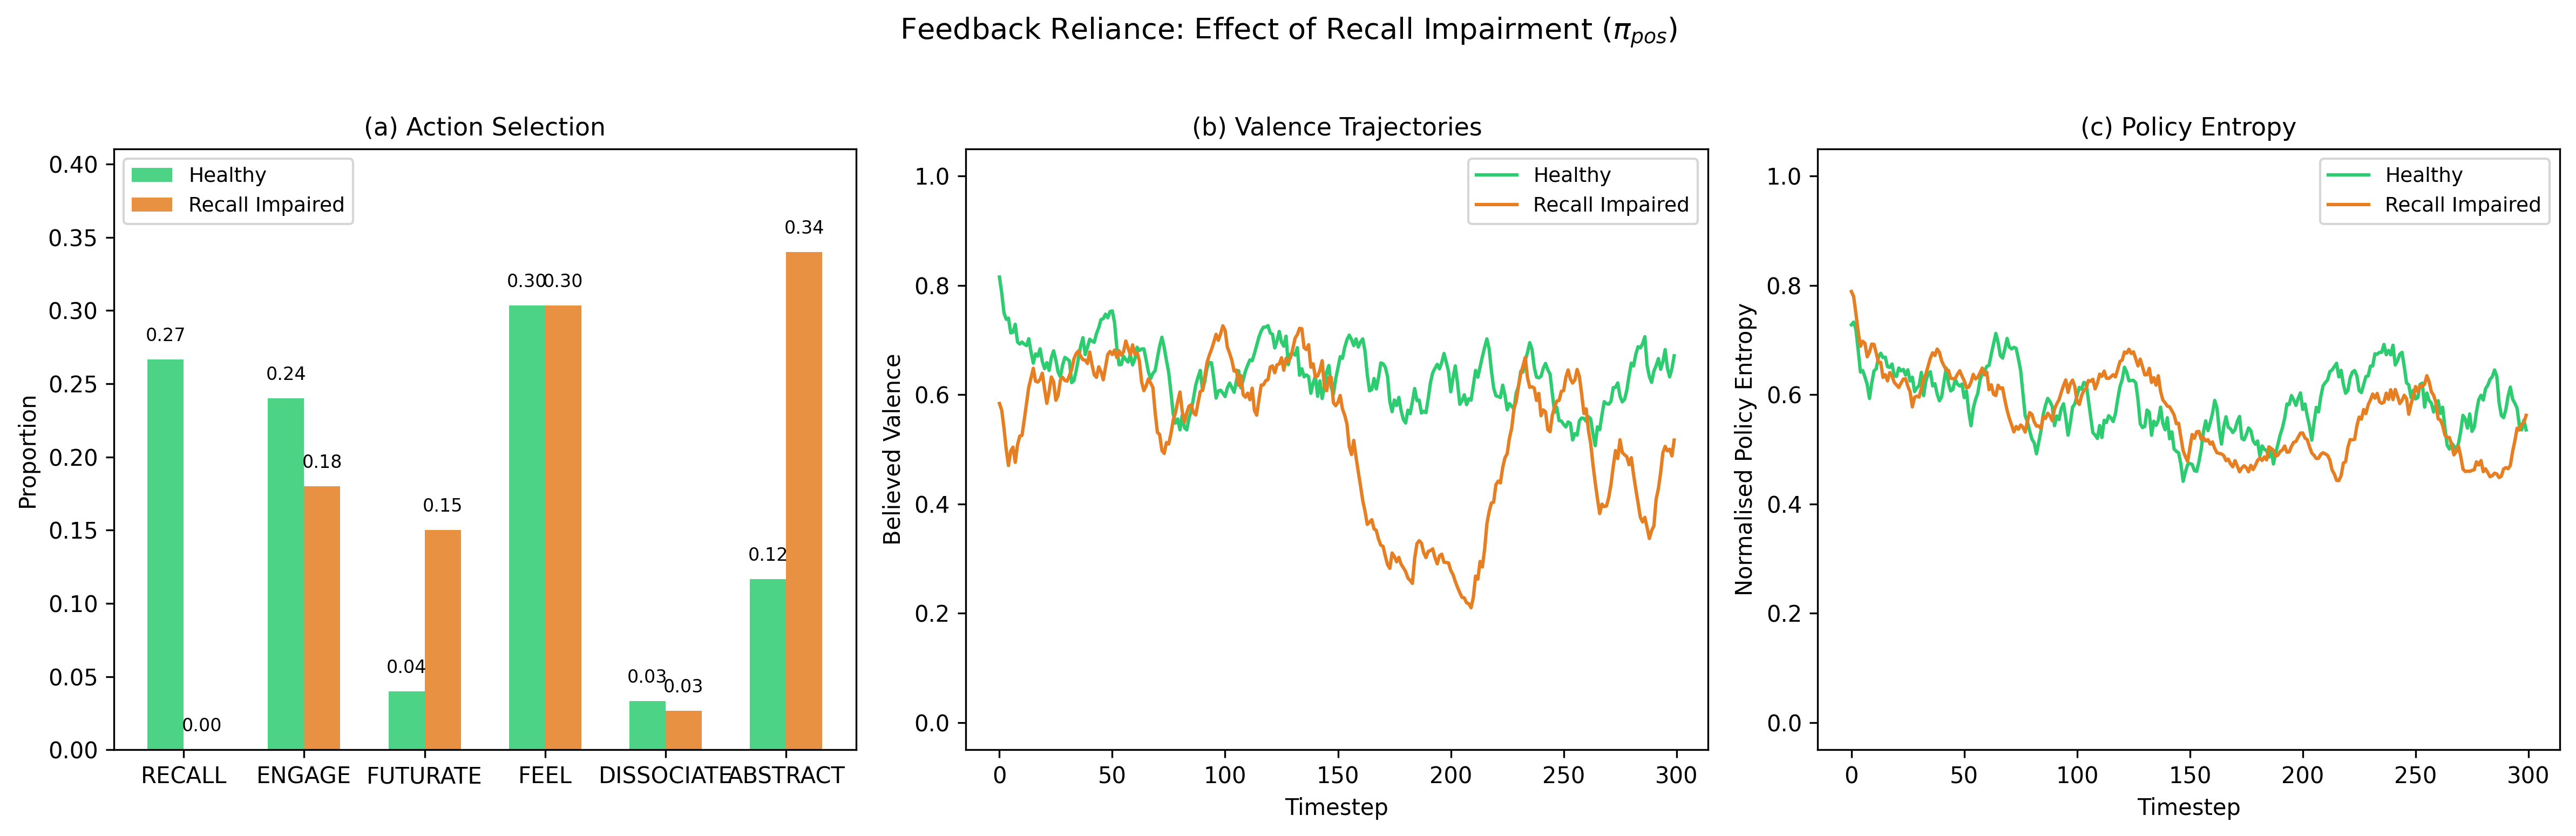
\includegraphics[width=\textwidth]{figures/fig10_feedback_reliance.png}
    \caption{\textbf{Feedback reliance under recall impairment.} Both profiles share $c_{\text{scale}} = 1.0$, $K = 8$, $\omega_e = 5.0$, $\gamma = 16$; they differ only in $\pi_{\text{pos}}$ (5.0 vs 0.2). (a) Action proportions: the recall-impaired agent's RECALL drops from 41\% to 7\%, with compensatory REST increase (59\% to 87\%) and emergent FUTURATE (0\% to 6\%). (b) Valence trajectories: recall impairment reduces mean valence ($0.52$ vs $0.63$) despite intact reward sensitivity. (c) Policy entropy: the recall-impaired agent is modestly less decisive.}
    \label{fig:feedback_reliance}
\end{figure}


\section{Future-Oriented Framing: Reactive Planning}\label{sec:future}

\subsection{Mechanism of FUTURATE}\label{sec:futurate_mechanism}

The FUTURATE policy redistributes precision toward anticipated future states. $\mathbf{B}_v^{\textsc{futurate}}$ pulls valence toward the solution state $K{-}1$ (50\% pull strength), modelling the generation of a highly precise prospective counterfactual. The energy cost is heavy ($-1.2$ per step), reflecting the metabolic expense of prospective simulation and active goal-directed behaviour. $\mathbf{B}_f^{\textsc{futurate}}$ is 90\% absorbing: once the agent enters future-oriented framing, narrative inertia keeps it there.

The EFE profile of FUTURATE is distinctive: it has the \emph{lowest} valence risk (because the $\mathbf{B}_v$ pull maximally aligns predicted observations with preferences) but the \emph{highest} energy risk (because of the metabolic cost). This tension between valence benefit and energy cost creates a natural brake on FUTURATE selection.

\subsection{Triggered by High Prediction Error}\label{sec:futurate_trigger}

When the agent's beliefs are far from preferred (high VFE), all policies have large risk terms. However, FUTURATE has the largest risk \emph{reduction} because $\mathbf{B}_v^{\textsc{futurate}}$ pulls most strongly toward the preferred state. The standard softmax $\pi(a) \propto \exp(-\gamma \cdot G(a))$ naturally selects FUTURATE when VFE is high, not as a heuristic but as an emergent consequence of the EFE decomposition.

Simulation evidence confirms this (Figure~\ref{fig:framing_dynamics}b, f). Mean VFE conditioned on selected action shows that FUTURATE is preferentially selected at higher-VFE timesteps than RECALL or ENGAGE. The VFE--$\pi(\text{FUTURATE})$ correlation is monotonically positive in healthy and manic agents, and flat in depressive agents (consistent with anhedonia rendering all policies similarly valued).

\subsection{Shorter Behavioural Horizons}\label{sec:short_horizon}

FUTURATE's energy cost creates a natural brake via EFE. After one to two steps of FUTURATE, the predicted interoceptive observation enters the ``depleted'' range, which increases the energy-modality risk term. The softmax shifts away from FUTURATE, producing short, reactive planning bursts rather than sustained commitment.

Simulation evidence (Figure~\ref{fig:framing_dynamics}c) confirms that FUTURATE runs are consistently shorter than RECALL runs: mean FUTURATE run length $\approx 1.3$ timesteps versus RECALL $\approx 1.7$ timesteps. The contrast is mechanistically transparent: RECALL has zero energy cost and therefore no brake, while FUTURATE's energy cost provides an inherent self-limiting mechanism. FUTURATE is therefore a reactive, bursty planning mode, not a sustained strategic commitment.

\subsection{Frame Beliefs and Temporal Orientation}\label{sec:frame_beliefs}

The posterior frame belief $q(f \mid o)$, obtained by marginalising the full posterior over valence and energy, provides a direct readout of the agent's believed temporal orientation. Healthy agents show balanced frame allocation ($\approx 0.30$ future, $\approx 0.45$ present, $\approx 0.25$ past), reflecting adaptive use of all temporal modes (Figure~\ref{fig:framing_dynamics}a). The three clinical phenotypes from the companion paper show qualitatively distinct profiles: manic agents have elevated future-frame belief ($\approx 0.4$--$0.5$), depressive agents have suppressed future-frame belief, and healthy agents maintain moderate balance.

\begin{figure}[htbp]
    \centering
    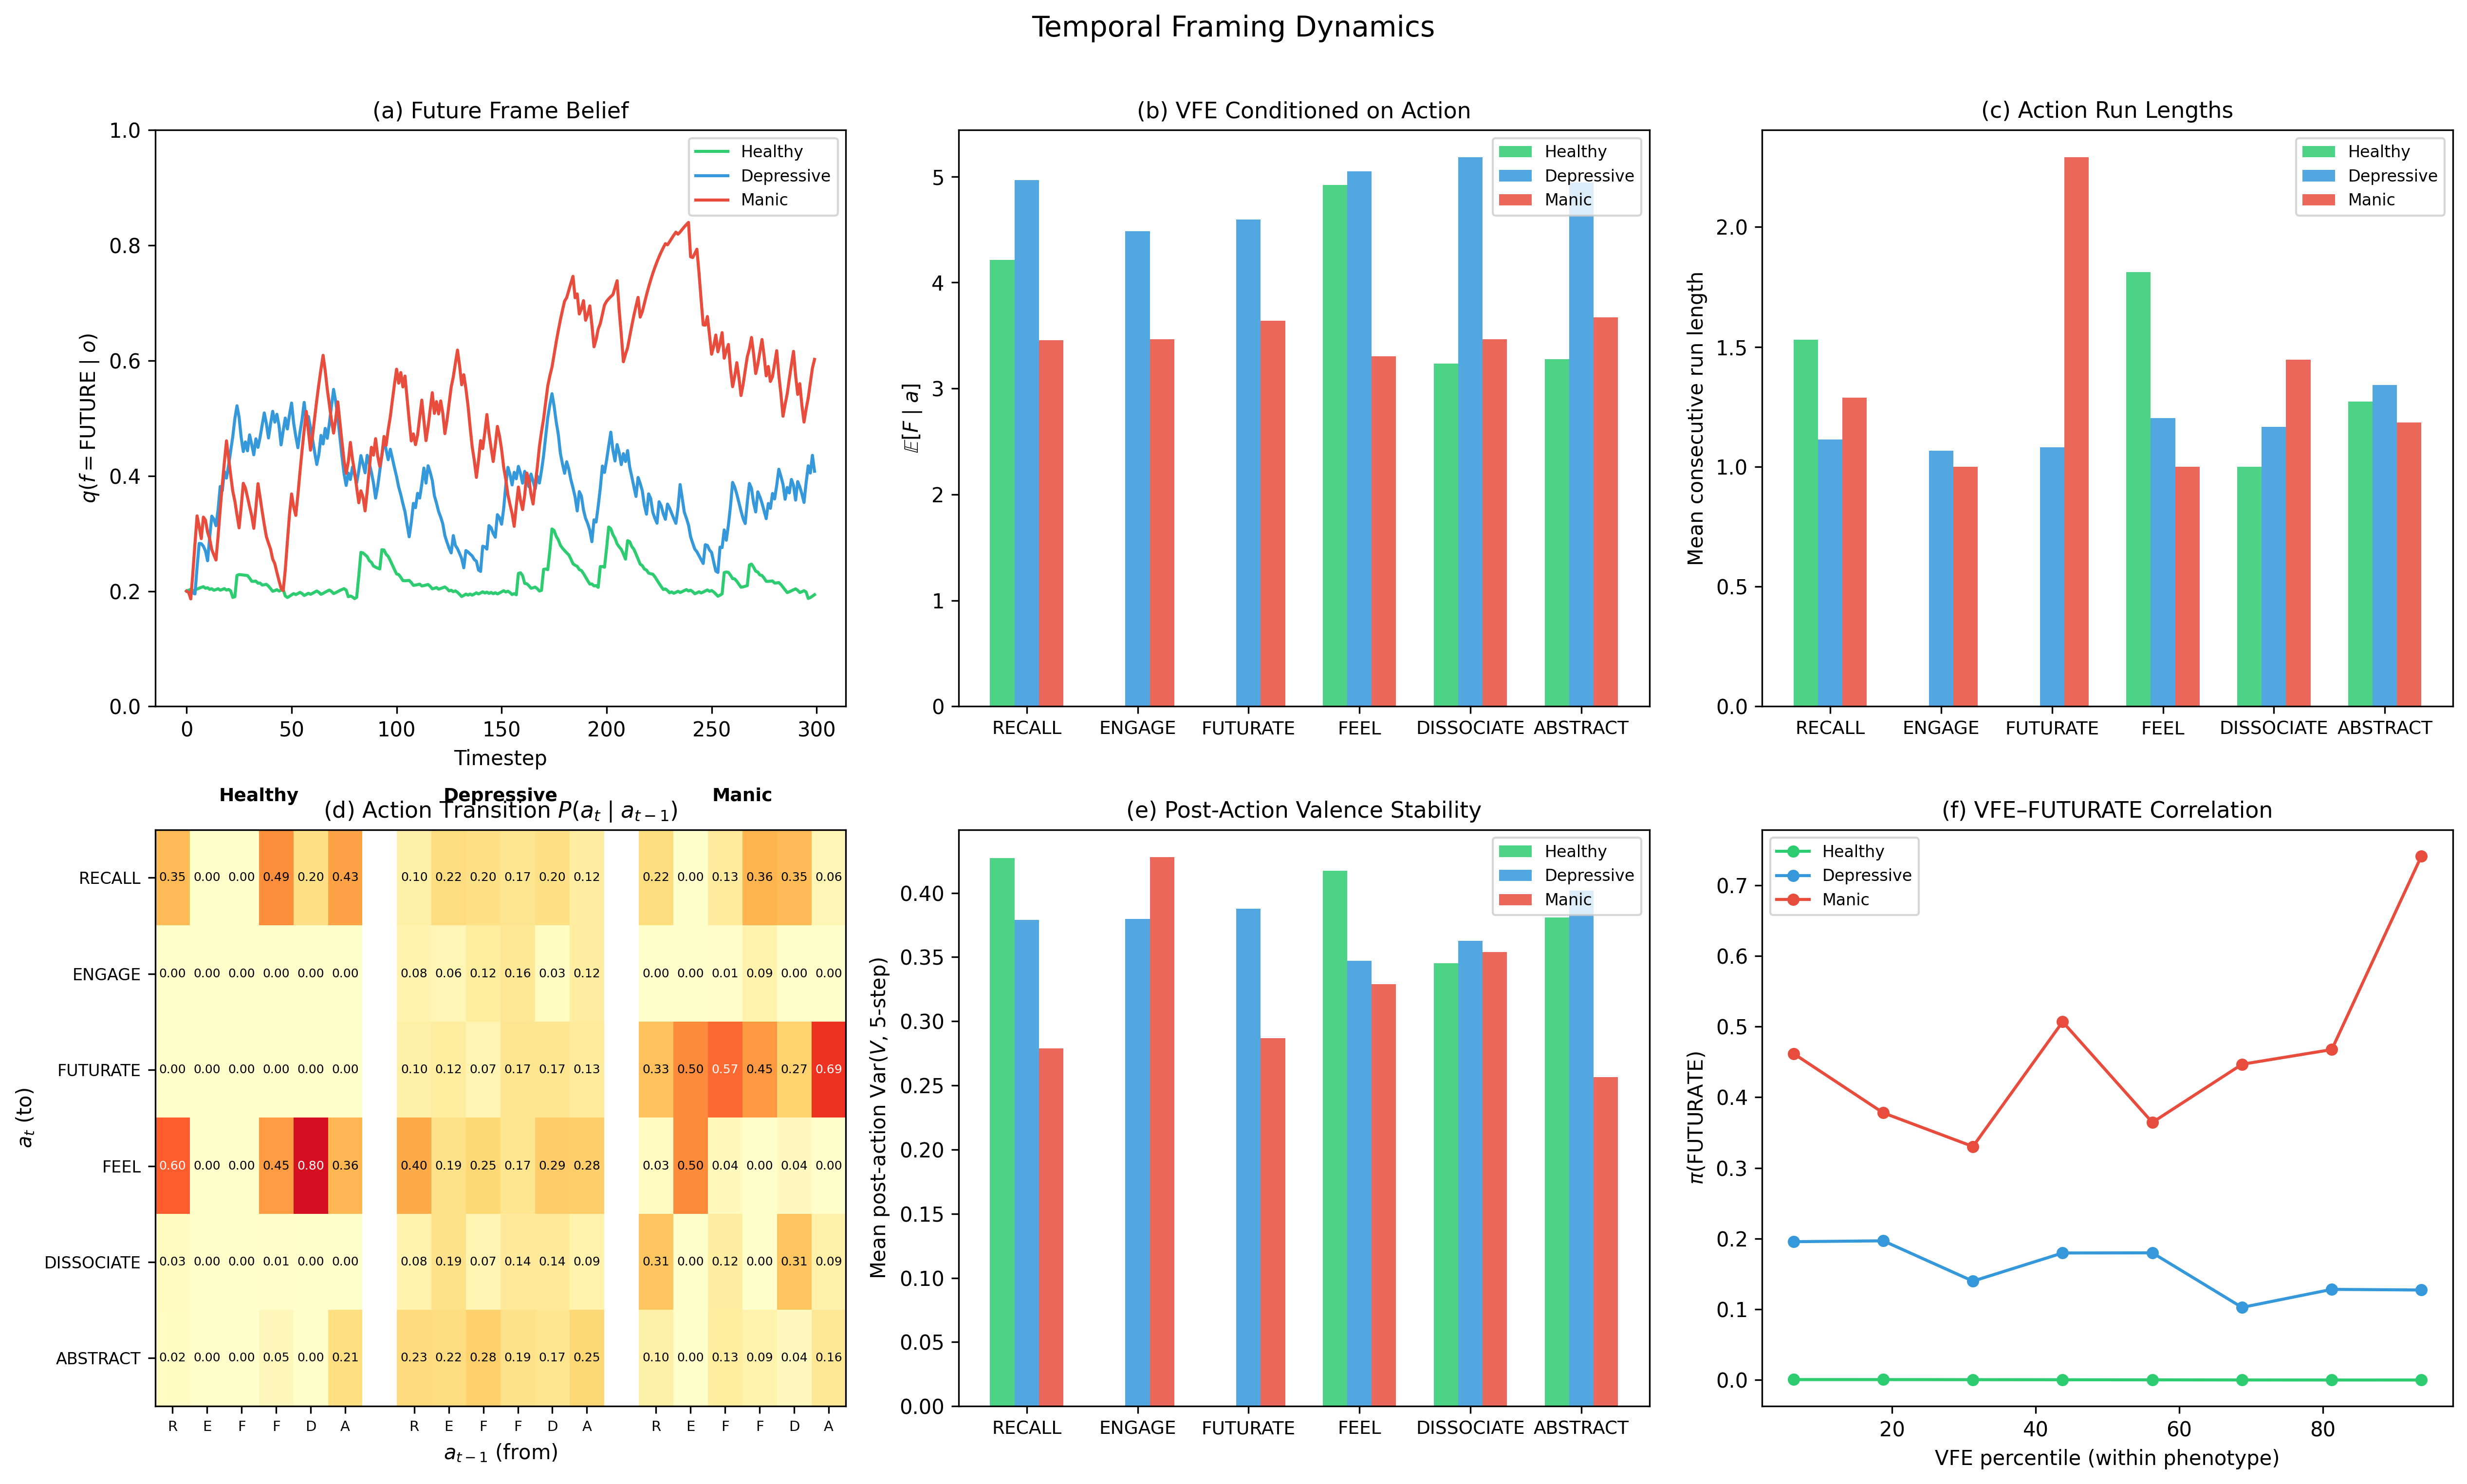
\includegraphics[width=\textwidth]{figures/fig11_framing_dynamics.png}
    \caption{\textbf{Temporal framing dynamics.} (a) Future frame belief $q(f{=}\textsc{future} \mid o)$ over time per phenotype, demonstrating differential temporal orientation. (b) Mean VFE conditioned on selected action: FUTURATE is preferentially selected at higher-VFE timesteps. (c) Mean action run length: FUTURATE runs are shorter than RECALL runs, reflecting reactive planning. (d) Action transition matrices $P(a_t \mid a_{t-1})$ per phenotype, showing the RECALL$\to$ENGAGE pipeline in healthy agents. (e) Post-action valence stability: 5-step rolling variance following each action; RECALL produces lower variance in healthy agents. (f) Binned VFE vs $\pi(\text{FUTURATE})$: monotonic positive relationship in healthy and manic agents, flat in depressive.}
    \label{fig:framing_dynamics}
\end{figure}


\section{Chronic Stress as Maladaptive Temporal Fixation}\label{sec:chronic_stress}

\subsection{Self-Regulation Versus Self-Amplification}\label{sec:self_reg}

The emotion--action--inference loop (\S\ref{sec:loop}) admits two dynamical regimes. Under \emph{self-regulation}, the loop is homeostatic: negative valence increases learning rate, which improves the model, which in turn produces positive valence \citep{joffily2013emotional}. This is the healthy default, in which prediction errors are informative signals that improve the model.

Under \emph{self-amplification}, the loop becomes pathological. When temporal framing locks into a single mode, precision on that mode's prediction errors increases, and the agent cannot update away from the locked frame. Chronic stress represents the self-amplifying pathology of temporal framing.

\subsection{The Pathological Cycle}\label{sec:pathological_cycle}

We introduce a ``stressed'' profile characterised by three concurrent perturbations from the healthy baseline: high environmental volatility ($0.7$ vs $0.3$), elevated reward sensitivity ($c_{\text{scale}} = 2.0$ vs $1.0$), and stress-impaired interoception ($\omega_e = 0.5$ vs $5.0$). The interoceptive impairment is clinically grounded: chronic stress is associated with reduced interoceptive accuracy \citep{barrett2017theory, seth2016interoceptive}.

These perturbations interact through the EFE decomposition in three reinforcing ways. First, impaired interoception ($\omega_e = 0.5$) blurs the agent's $\mathbf{A}_{\text{int}}$ matrix, reducing the energy-modality risk term that would normally deter FUTURATE selection; in effect, the brake is disabled. Second, elevated reward sensitivity ($c_{\text{scale}} = 2.0$) amplifies the preference vectors $\mathbf{C}$, increasing the valence-modality risk reduction for FUTURATE; the accelerator is enhanced. Third, under the standard softmax policy selection $\pi(a) \propto \exp(-\gamma \cdot G(a))$, FUTURATE naturally enters the policy mix when the brake is disabled and the accelerator is enhanced.

Once FUTURATE enters the policy mix, its 90\% absorbing frame transition creates narrative inertia, causing the agent to persist in future-oriented framing. The volatile environment then keeps violating the agent's precise future predictions, producing chronic positive $\Delta F$ (increasing VFE). This creates the self-amplifying cycle: FUTURATE produces precise predictions, which the environment violates, producing negative $v_{\text{model}}$, which elevates VFE and further favours FUTURATE (\S\ref{sec:futurate_trigger}).

\subsection{Temporal Dysregulation Pattern}\label{sec:temporal_dysreg}

The stressed agent's posterior frame belief shows a characteristic pattern: elevated \textsc{past} (from compensatory RECALL) and elevated \textsc{future} (from FUTURATE), with depleted \textsc{present} (Figure~\ref{fig:chronic_stress}a). The agent oscillates between rumination (RECALL) and overmentalising (FUTURATE), never settling in present engagement.

This pattern of elevated temporal extremes with depleted present is the computational signature of temporal dysregulation. It maps onto the clinical presentation of chronic stress and anxiety disorders, where patients report excessive past-oriented rumination and future-oriented worry at the expense of present-moment awareness \citep{berg2022rumination}.

\subsection{Persistent Backward Negative Valence}\label{sec:backward_negative}

The stressed agent's backward valence $v_{\text{model}} = \tanh(-\Delta F / \tau)$ is persistently more negative than the healthy agent's (Figure~\ref{fig:chronic_stress}b). The mechanism is precise: the volatile environment keeps violating the agent's predictions (producing positive $\Delta F$), so the backward channel, which evaluates how well past predictions matched observations, is persistently negative.

FUTURATE exacerbates this effect. By pulling beliefs toward the solution state, FUTURATE creates \emph{precise predictions about positive future outcomes} that the volatile environment then violates, amplifying $\Delta F$. The backward negative valence is therefore not a belief about the past being bad, but a \emph{signal} that the model's fit to recent observations is deteriorating, a signal amplified by the very mechanism (FUTURATE) that the agent uses to cope.

\subsection{Channel Decomposition}\label{sec:channel_decomp}

The stressed agent's valence channel decomposition reveals the full temporal structure of chronic stress (Figure~\ref{fig:chronic_stress}c). The backward channel ($v_{\text{model}}$) is persistently negative, reflecting chronic model violations from the volatile environment amplified by FUTURATE's precise predictions. The reward channel ($v_{\text{reward}}$) oscillates around zero, as the volatile environment produces unpredictable reward prediction errors that are sometimes good, sometimes bad, but never stable. The action channel ($v_{\text{action}}$) shows intermittent positive bursts: the agent keeps finding ``better'' policies under high VFE (policy improvement is easy when the current policy is poor), but the improvement is ephemeral because the environment keeps changing.

This pattern of persistent backward negativity, oscillating present, and ephemeral forward positivity is the computational signature of overmentalising: optimistic planning followed by systematic model-fit deterioration.

\begin{figure}[htbp]
    \centering
    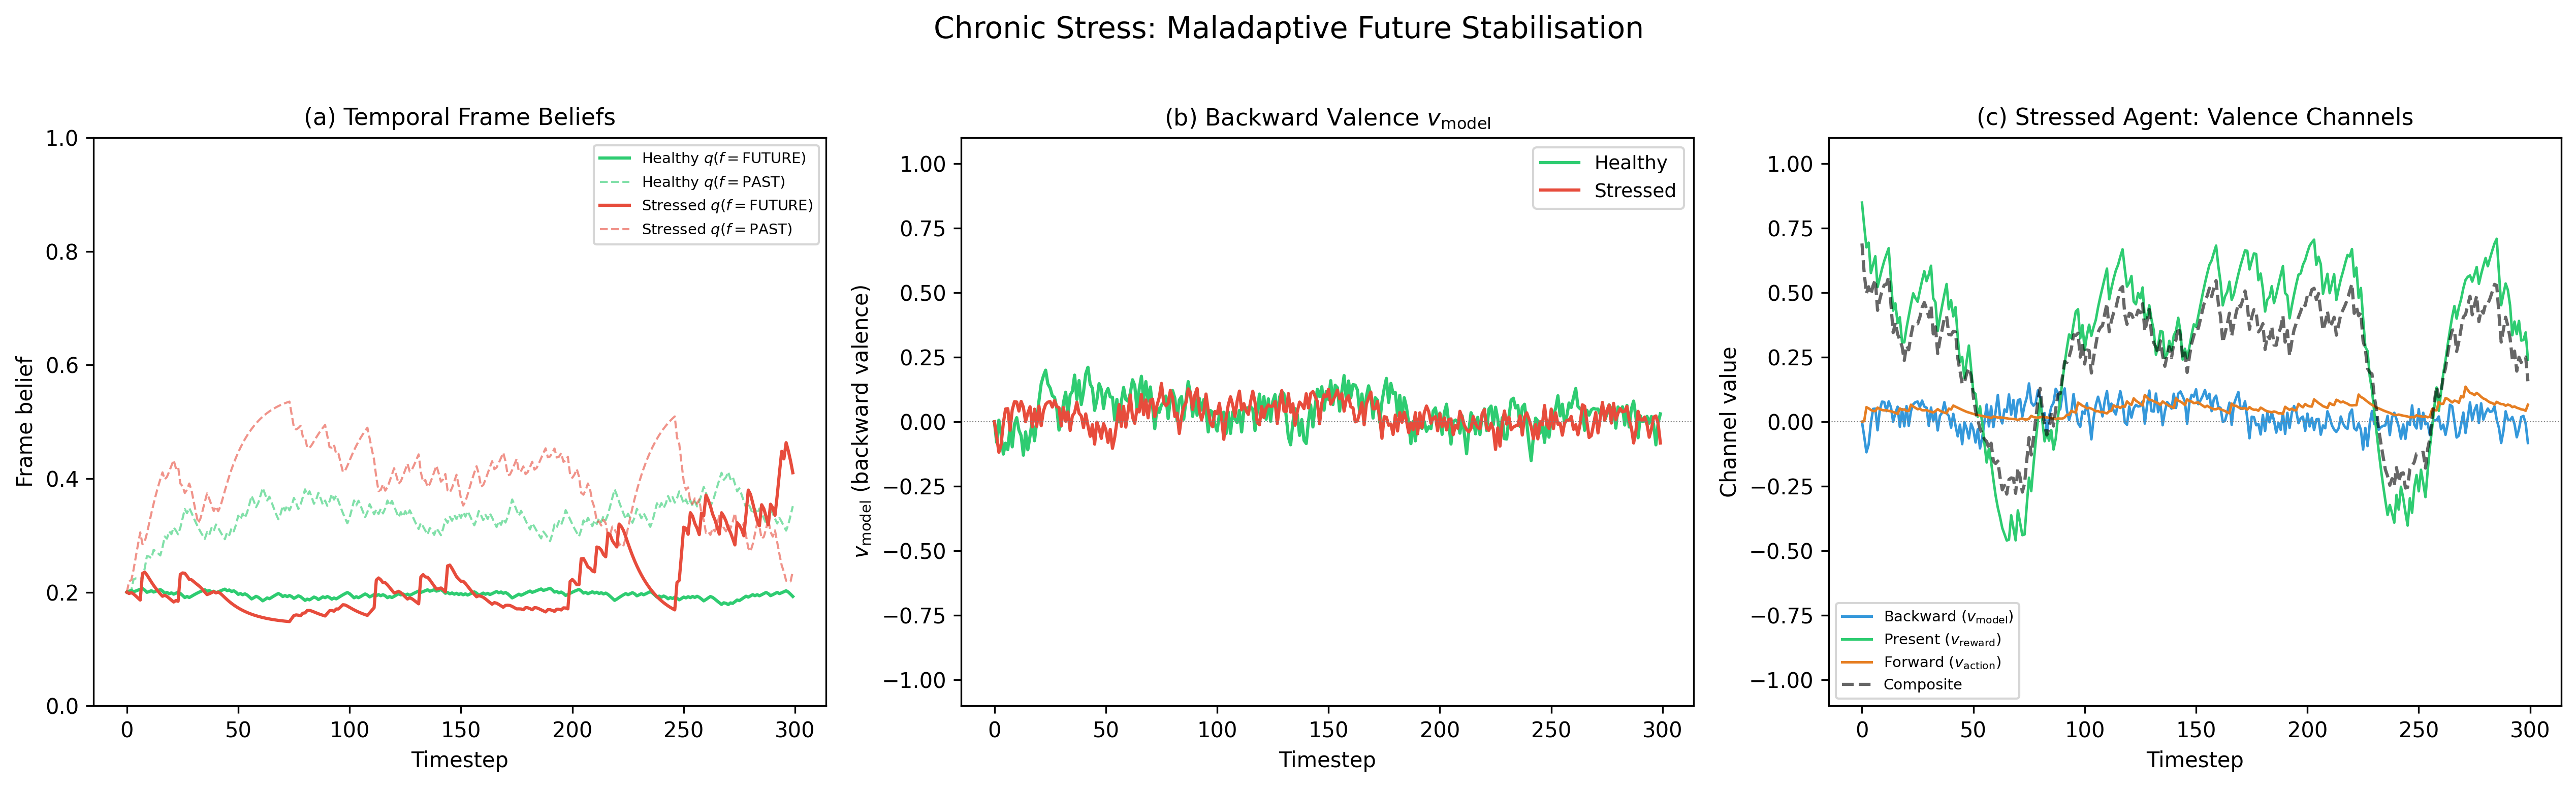
\includegraphics[width=\textwidth]{figures/fig12_chronic_stress.png}
    \caption{\textbf{Chronic stress as maladaptive temporal fixation.} Stressed profile ($c_{\text{scale}} = 2.0$, $\omega_e = 0.5$, volatility $= 0.7$) vs healthy ($c_{\text{scale}} = 1.0$, $\omega_e = 5.0$, volatility $= 0.3$); $K{=}8$, $\pi_{\text{pos}} = 3.0$, $\gamma = 16$ shared. (a)~Frame beliefs: the stressed agent shows elevated FUTURE and PAST frame beliefs with depleted PRESENT (temporal dysregulation). (b)~Backward valence $v_{\text{model}}$: more variable and persistently negative in the stressed agent (chronic model-fit deterioration from high volatility). (c)~Valence channel decomposition for the stressed agent: backward channel persistently negative, reward channel oscillating, action channel showing intermittent positive bursts.}
    \label{fig:chronic_stress}
\end{figure}


\section{Discussion}\label{sec:discussion}

\subsection{Temporal Aiming as a Unified Theory}\label{sec:unified_theory}

This paper has formally proposed what has been implicit in the active inference literature but never unified in a single account: the VFE/EFE distinction provides a natural temporal taxonomy of emotion. Variational free energy concerns beliefs about what \emph{has happened} and generates backward-oriented affect (regret, guilt, pride, gratitude). Expected free energy concerns expectations about what \emph{will happen} and generates forward-oriented affect (hope, fear, anxiety, anticipation). The rate of change at the current moment generates present-oriented affect (joy, anger, surprise). Transitional emotions (relief, disappointment) arise from comparing current VFE with prior EFE predictions.

Counterfactual temporal framing is the \emph{mechanism} by which agents actively navigate this temporal structure. Different from \citet{hinrichs2025temporal}, who addressed temporal aiming in dyadic interaction, we have addressed the single-agent computational mechanism: temporal framing as precision redistribution across temporal horizons, naturally selected by EFE minimisation.

\subsection{Temporal Framing as a General Mechanism}\label{sec:general_mechanism}

Temporal framing is not specific to pathology. Healthy agents \emph{use} temporal framing for adaptive regulation: RECALL stabilises affect (creating a floor under valence), FUTURATE provides reactive planning (responding to high prediction error), and the natural energy cost of FUTURATE provides a self-limiting brake. Pathology arises not from temporal framing itself but from the failure of its balancing mechanisms, whether the brake is disabled (impaired interoception), the accelerator is enhanced (reward hypersensitivity), or the stabiliser fails (impaired positive-belief precision).

\subsection{Connection to Attention-as-Precision}\label{sec:attention_connection}

\citet{feldman2010attention} established that attention is precision weighting on prediction errors. Our framework extends this to the temporal domain: \emph{temporal attention} is precision weighting on temporal horizons. The $\mathbf{B}_{\text{frame}}$ matrices function as temporal attention operators, and action selection in the temporal framing domain amounts to deciding \emph{where in time} to attend. This connects temporal framing to the broader predictive processing literature on selective attention, suggesting that spatial attention (``where to look'') and temporal attention (``when to think about'') are instances of the same precision-weighting mechanism applied to different dimensions of the generative model.

\subsection{Mood Versus Emotion Timescales}\label{sec:mood_emotion}

\citet{hesp2021deeply} distinguished two timescales in the affect hierarchy: M4 (emotion), operating within-trial as fast precision dynamics, and M5 (mood), operating cross-trial as slow valence state inference. Temporal framing operates at the \emph{interface} between these timescales. Individual frame selections are M4 phenomena, reflecting fast, within-trial decisions about temporal orientation driven by current EFE. Sustained frame biases are M5 phenomena, reflecting slow, cross-trial tendencies toward particular temporal orientations that encode learned or dispositional patterns.

The transition from adaptive temporal framing (M4) to chronic temporal fixation (M5) is precisely the self-amplification pathology described in \S\ref{sec:chronic_stress}. A future extension would make this hierarchy explicit, with frame selection at the lower level and frame \emph{policy} at the higher level, capturing the dynamics of narrative entrenchment and therapeutic flexibility \citep{hein2022emotion}.

\subsection{Relationship to Bipolar Disorder}\label{sec:bipolar_connection}

Our companion paper \citep{albarracin2026bipolar} models bipolar disorder as pathology of energy $\times$ interoception, with clinical phenotypes emerging from parameter variation along four dimensions ($\pi_{\text{pos}}$, $K$, $\omega_e$, $c_{\text{scale}}$). The present paper provides the \emph{general temporal mechanism} that bipolar disrupts. Bipolar disorder involves pathological \emph{cycling} of temporal frames: manic episodes are locked FUTURATE (aggressive future-oriented framing that depletes energy), crashes are forced REST (energy recovery), and depressive episodes involve failed temporal flexibility (inability to select any adaptive frame). Chronic stress, by contrast, involves pathological \emph{fixation} without cycling: the agent oscillates between RECALL and FUTURATE without the energy crash that forces reset.

\subsection{Depression as Failed Temporal Flexibility}\label{sec:depression}

Depression can be understood as the failure of temporal flexibility. \citet{krupnik2021depression} proposed that depression may represent ``failed anxiety,'' the inability to mount even an anxious (forward-oriented) response to threat. In our framework, this corresponds to precision collapse: the depressive agent's anhedonia ($c_{\text{scale}} \to 0$) flattens the EFE landscape so thoroughly that no temporal frame is favoured over any other. The result is not temporal fixation (as in chronic stress) but temporal \emph{incoherence}, with uncertainty diffusely distributed across all horizons and the agent unable to commit to any temporal orientation.

The depressive agent's near-random policy is the computational signature of this incoherence: the agent cannot decide whether to look backward, engage with the present, or plan for the future. Therapeutic interventions that restore precision on any single temporal dimension (e.g., behavioural activation for the present, or structured reminiscence for the past) may bootstrap recovery by providing a seed of temporal coherence from which adaptive regulation can rebuild.

\subsection{Limitations and Future Directions}\label{sec:limitations}

Several limitations point toward future work. First, the current model treats temporal framing as a single-step policy selection rather than a deep temporal hierarchy \citep{friston2018deep}. Extending to a hierarchical POMDP, with temporal frame inferred at a higher level, would capture narrative entrenchment and flexibility more naturally.

Second, the temporal frame is modelled as a categorical variable ($\{$\textsc{past}, \textsc{present}, \textsc{future}$\}$) rather than a continuous temporal depth. In reality, ``the past'' admits degrees, from last week to childhood, and temporal framing may involve selecting a continuous temporal horizon rather than a discrete category.

Third, the $\mathbf{B}_{\text{frame}}$ matrices are fixed rather than learned. An agent that could learn its own temporal attention operators would develop personalised temporal framing strategies, potentially capturing individual differences in temporal orientation as learned generative model parameters.

Fourth, the M4/M5 hierarchy is discussed but not implemented. An explicit mood layer would capture the dynamics of sustained temporal biases (dispositional optimism, chronic rumination) as slow parameters of the generative model, following \citet{hesp2021deeply} and \citet{pezzulo2018hierarchical}.

Finally, the model addresses single-agent temporal framing. Extending to dyadic and multi-agent settings, where agents' temporal frames interact and potentially synchronise, would connect to the temporal aiming literature in social cognition \citep{hinrichs2025temporal} and to the broader project of understanding how shared temporal orientation supports interpersonal coordination \citep{eldar2016mood}.

\bibliographystyle{plainnat}
\bibliography{references}

\end{document}
